\documentclass[a4paper,13pt]{article}
\usepackage[utf8]{inputenc}
\usepackage[T5]{fontenc} 
\usepackage[fontsize=13pt]{scrextend} 
\usepackage[paperheight=29.7cm, paperwidth=21cm, right=15mm,left=25mm,top=20mm,bottom=20mm]{geometry} % Chuẩn A4, căn lề phải, trái, trên, dưới
\usepackage{biblatex}
\addbibresource{references.bib} 
\usepackage{media9}
\usepackage{mathptmx} 
\usepackage{comment}
\usepackage{graphicx} 
\usepackage{float} 
\usepackage{hyperref}
\usepackage{tikz} 
\usetikzlibrary{calc} 
\usepackage{xcolor} 
\usepackage{colortbl} 
\usepackage{array} 
\usepackage{lettrine} 
\usepackage{multicol} 
\usepackage{tocloft} 
\usepackage{booktabs}  
\usepackage[labelformat=empty]{caption}
\usepackage{hyperref} 
\usepackage{bookmark} 
\usepackage{titletoc}
\usepackage{amsmath}
\usepackage{fancyhdr}
\usepackage{bibentry}
\pagestyle{fancy}
\usepackage{utopia}
\usepackage{listings}

\renewcommand*{\bibfont}{\small}
\renewcommand{\thesection}{\Roman{section}}

% Tạo header và footer
\fancyhf{}
\chead{\textbf{\textit{ĐIỀU CHẾ ADC}}}
\lfoot{\textbf{\textit{SVTH: Nguyễn Bá Thành - Võ Đức Hiếu \hspace{2cm} Hướng dẫn: TS.Võ Duy Phúc}}}
\rfoot{\thepage}
\renewcommand{\headrulewidth}{1pt}
\renewcommand{\footrulewidth}{1pt}


\thispagestyle{empty}

% Tùy chỉnh mục lục bảng và hình ảnh
\renewcommand{\cftsubsecpresnum}{}
\renewcommand{\listfigurename}{}
\renewcommand{\listtablename}{}

% Tùy chỉnh định dạng mục lục hình ảnh và bảng
\renewcommand{\cftfigpresnum}{Hình }
\renewcommand{\cftfigaftersnum}{: }
\setlength{\cftfignumwidth}{1cm}

\renewcommand{\cfttabpresnum}{Bảng }
\renewcommand{\cfttabaftersnum}{: }
\setlength{\cfttabnumwidth}{1cm}

\lstset{
  language=Matlab,
  basicstyle=\ttfamily\small,
  keywordstyle=\color{blue},
  commentstyle=\color{gray},
  stringstyle=\color{red},
  numbers=left,
  numberstyle=\tiny\color{gray},
  stepnumber=1,
  numbersep=5pt,
  backgroundcolor=\color{white},
  frame=single,
  breaklines=true,
  captionpos=b,
  tabsize=2,
  keepspaces=true,         % ⚠️ Giữ nguyên khoảng trắng và tab
  showstringspaces=false,  % Ẩn dấu cách trong chuỗi
  columns=flexible         % ⚠️ Giúp xử lý ký tự _ và khoảng trắng tốt hơn
}

\begin{document}
\renewcommand{\thesection}{}
\renewcommand{\thesubsection}{}
\begin{titlepage}
\begin{tikzpicture}[overlay,remember picture]
\draw [line width=3pt]
($ (current page.north west) + (2.5cm, -1.5cm) $)
rectangle
($ (current page.south east) + (-1.5cm, 1.5cm) $);
\draw [line width=0.5pt]
($ (current page.north west) + (2.4cm, -1.6cm) $)
rectangle
($ (current page.south east) + (-1.4cm, 1.6cm) $);
\end{tikzpicture}

\begin{center}
\vspace{-6pt}
\textbf{\fontsize{18pt}{0pt}\selectfont ĐẠI HỌC ĐÀ NẴNG} \\
\textbf{\fontsize{18pt}{0pt}\selectfont TRƯỜNG ĐẠI HỌC BÁCH KHOA} \\
\textbf{\fontsize{18pt}{0pt}\selectfont KHOA ĐIỆN TỬ - VIỄN THÔNG}
\end{center}

\begin{center}
\begin{figure}[H]
    \centering
    \includegraphics[scale=0.5]{logo.jpg} % Giảm kích thước ảnh xuống 50%
    \label{fig:logo_scale}
\end{figure}
\end{center}

\begin{center}
\textbf{\fontsize{30pt}{0pt}\selectfont BÁO CÁO CUỐI KÌ PBL4}  \\ 
\vspace{15pt}
%\textbf{\fontsize{17pt}{0pt}\selectfont MÔN HỌC: Mạng và hệ thống truyền thông tiên tiến} \\
\vspace{30pt}
\textbf{\fontsize{15pt}{0pt}\selectfont ĐỀ TÀI:} \\ 
\vspace{15pt}
\fontsize{20pt}{0pt}\selectfont ĐIỀU CHẾ ADC
\end{center}
\vspace{40pt}

\begin{flushleft}
\hspace{4cm}Sinh viên thực hiện \hspace{0.05cm}: Nguyễn Bá Thành \\
\hspace{8.13cm}: Võ Đức Hiếu \\
\hspace{4cm}Lớp \hspace{3.2cm}: 21DTCLC4 \\
\hspace{4cm}Nhóm \hspace{2.7cm}: 21.40 \\
%\hspace{4cm}MSSV \hspace{2.7cm}: 106210200 \\
\hspace{4cm}Giảng viên \hspace{1.8cm}: TS.Võ Duy Phúc \\
\end{flushleft}
\vspace{3cm}
\begin{center}
    \textit{Tháng 6 năm 2025}
\end{center}
\end{titlepage}

\begin{center}
\section{TÓM TẮT}
\end{center}
Điều chế ADC hay Analog-to-Digital Converter là một thành phần quan trọng trong hệ thống viễn thông hiện đại. ADC là thiết bị điện tử chuyển đổi tín hiệu analog (liên tục) thành tín hiệu digital (rời rạc), cho phép các hệ thống digital xử lý và truyền tải thông tin từ thế giới thực. ADC có nhiều loại kiến trúc khác nhau như: \\

\begin{itemize}
    \item Successive Approximation Register (SAR) ADC: Có độ chính xác tốt, tiêu thụ điện năng thấp và tốc độ vừa phải. Ứng dụng trong đo lường, thiết bị IoT, cảm biến, hệ thống nhúng.
    \item Delta-Sigma ADC: Độ phân giải rất cao, khả năng lọc nhiễu tốt. Sử dụng trong âm thanh số, y tế, thiết bị đo chính xác cao.
    \item Flash ADC: Tốc độ rất cao, độ trễ thấp nhưng tiêu thụ điện năng lớn, tốn diện tích. Được dùng trong radar, thu phát RF, xử lý tín hiệu tốc độ cao.
    \item Dual slope: Chính xác, ít bị nhiễu, đơn giản nhưng tốc độ chậm. Nên được dùng trong máy đo đa năng (multimeter), thiết bị đo lường chính xác.
    \item Pipelined: Cân bằng giữa tốc độ và độ phân giải nhưng độ trễ cao hơn Flash, phức tạp hơn SAR. Dùng cho xử lý tín hiệu ảnh, video, thu nhận dữ liệu tốc độ cao.
\end{itemize}

Tại Việt Nam, ngành viễn thông đang phát triển nhanh chóng với sự chuyển đổi số mạnh mẽ. Theo \href{https://www.mordorintelligence.com/industry-reports/data-converter-market}{\textbf{ Mordor Intelligence}}, thị trường viễn thông Việt Nam dự kiến sẽ tăng trưởng với tốc độ CAGR 1.21\% trong giai đoạn 2024-2029, và sự phát triển này sẽ đi kèm với nhu cầu cao hơn về ADC. Các nhà mạng lớn như Viettel, Vinaphone, và Mobifone đang đầu tư mạnh vào cơ sở hạ tầng số, bao gồm triển khai công nghệ 5G và mở rộng hạ tầng cáp quang. \\

Trên toàn cầu, thị trường ADC đang phát triển mạnh mẽ, đặc biệt trong bối cảnh công nghệ 5G và IoT. Theo báo cáo của \href{https://www.grandviewresearch.com/industry-analysis/antibody-drug-conjugates-market}{\textbf{ Grand View Research}}, thị trường ADC toàn cầu được dự báo sẽ đạt 10.5 tỷ USD vào năm 2025, với tốc độ tăng trưởng CAGR 7.8\% từ 2020 đến 2025. \\

Với độ phân giải cao hơn để xử lý tín hiệu phức tạp cùng với tốc độ chuyển đổi nhanh hơn để đáp ứng yêu cầu truyền tải dữ liệu lớn và tốc độ lấy mẫu có thể lên đến 250 kS/s thì điều chế ADC là một thành phần quan trọng trong hệ thống viễn thông hiện đại, đóng góp vào sự phát triển của ngành công nghệ số ở Việt Nam và trên toàn thế giới.
\vspace{2cm}
\clearpage  

\begin{center}
\section{LỜI NÓI ĐẦU VÀ CẢM ƠN}
\end{center}

Trong những thập kỷ gần đây, Việt Nam đang bước vào một kỷ nguyên phục hưng công nghệ đầy mạnh mẽ, từng bước khẳng định vị thế của mình trên bản đồ công nghệ thế giới. Từ một nền kinh tế chủ yếu dựa vào nông nghiệp, đất nước đã có những chuyển mình sâu sắc để trở thành một trung tâm công nghệ năng động, với những bước tiến vững chắc trong các lĩnh vực như viễn thông, công nghệ thông tin và các công nghệ tiên tiến mới nổi.\\

Trong dòng chảy đổi mới đó, công nghệ chuyển đổi tương tự – số (ADC - Analog to Digital Converter) và các kỹ thuật điều chế liên quan đang dần trở thành một trong những hướng phát triển trọng điểm, mở ra tiềm năng ứng dụng to lớn không chỉ trong ngành viễn thông, mà còn trong tự động hóa, y sinh, công nghệ quốc phòng và các hệ thống nhúng thông minh. \\

Tại Việt Nam, nhiều tập đoàn công nghệ lớn như VNPT, Viettel và FPT đang đầu tư mạnh mẽ vào nghiên cứu và ứng dụng các giải pháp dựa trên công nghệ ADC. Đồng hành cùng định hướng quốc gia đó, Trường Đại học Bách khoa – Đại học Đà Nẵng, với bề dày truyền thống đào tạo và nghiên cứu kỹ thuật, đang đóng vai trò nòng cốt trong việc đào tạo nguồn nhân lực chất lượng cao.\\

Trước hết, chúng em xin bày tỏ lòng biết ơn sâu sắc đến thầy \href{https://scv.udn.vn/vdphuc}{T.S Võ Duy Phúc}, người đã tận tình hướng dẫn và đồng hành cùng em trong suốt quá trình nghiên cứu và hoàn thiện đề tài. Những kiến thức chuyên môn, sự hỗ trợ quý báu và tinh thần khích lệ từ thầy là nguồn động lực lớn để chúng em vượt qua những khó khăn trong quá trình thực hiện.\\

Chúng Em xin gửi lời cảm ơn chân thành đến khoa \href{http://ete.dut.udn.vn/}{Điện tử - Viễn thông} và ban lãnh đạo Trường Đại học Bách khoa – Đại học Đà Nẵng đã tạo điều kiện thuận lợi cả về cơ sở vật chất lẫn môi trường học thuật để chúng em có cơ hội tiếp cận và phát triển chuyên môn trong lĩnh vực công nghệ tiên tiến.\\

Cuối cùng, chúng em hy vọng rằng đề tài này sẽ đóng góp một phần nhỏ vào kho tàng tri thức kỹ thuật, đồng thời là bước đệm cho các nghiên cứu chuyên sâu hơn trong tương lai, góp phần vào sự phát triển bền vững của nền công nghệ Việt Nam.\\

\textbf{\hspace{7cm} Đà Nẵng, ngày 12 tháng 6 năm 2025}\\

\textbf{\hspace{9cm} Người thực hiện}\\

\hspace{7cm} Nguyễn Bá Thành - Võ Đức Hiếu \\
\clearpage  
\begin{center}
\section{LỜI CAM ĐOAN LIÊM CHÍNH HỌC THUẬT}
\end{center}

Chúng em xin cam đoan rằng toàn bộ nội dung trong báo cáo/luận văn/đề tài này là kết quả của quá trình học tập, nghiên cứu và thực hiện của riêng chúng em dưới sự hướng dẫn của giảng viên hướng dẫn.\\

Chúng em hoàn toàn chịu trách nhiệm về tính trung thực và liêm chính học thuật của báo cáo này. Các số liệu, kết quả, hình ảnh và trích dẫn trong báo cáo đều được trình bày một cách trung thực, có nguồn gốc rõ ràng và tuân thủ đúng các quy định về đạo đức nghiên cứu và trích dẫn tài liệu.\\

Chúng em khẳng định rằng không sao chép, đạo văn hay sử dụng bất kỳ hình thức gian lận học thuật nào trong quá trình thực hiện báo cáo. Nếu phát hiện có bất kỳ hành vi vi phạm nào liên quan đến bản quyền hoặc tính trung thực học thuật, tôi xin hoàn toàn chịu trách nhiệm trước nhà trường và pháp luật.\\

\textbf{\hspace{7cm} Đà Nẵng, ngày 12 tháng 6 năm 2025}\\

\textbf{\hspace{9cm} Người cam đoan} \\

\hspace{7cm} Nguyễn Bá Thành - Võ Đức Hiếu \\

\clearpage 
\begin{center}
\section{MỤC LỤC}
\end{center}

\renewcommand{\contentsname}{}
\tableofcontents % Tạo mục lục
\clearpage

\begin{center}
\section{DANH MỤC HÌNH ẢNH}
\renewcommand{\listfigurename}{}
\listoffigures
\end{center}



\clearpage
\begin{table}[h]
    \centering
    \section{DANH SÁCH TỪ VIẾT TẮT}
    \begin{tabular}{lll}
        \toprule
        \textbf{Từ viết tắt} & \textbf{Tiếng Anh} & \textbf{Nghĩa tiếng Việt} \\
        \midrule
        ADC & Analog to Digital Converter & Bộ chuyển đổi tương tự sang số \\
        DAC & Digital to Analog Converter & Bộ chuyển đổi số sang tương tự \\
        DSP & Digital Signal Processing & Xử lý tín hiệu số \\
        SNR & Signal to noise ratio & Tỷ lệ tín hiệu trên nhiễu \\
        SQNR & Signal to quantization noise ratio & Tỷ lệ tín hiệu trên nhiễu lượng tử \\
        SINAD & Signal to Noise and Distortion & Tỷ lệ tín hiệu trên nhiễu và méo \\
        SAR & Successive Approximation Register & Thanh ghi xấp xỉ liên tiếp \\
        ENOB & Effective number of bits & Số bit hiệu quả \\
        SFDR & Spurious Free Dynamic Range & Dải động không có tín hiệu giả \\
        INL & Integral Nonlinearity & Sai số không tuyến tính tích phân \\
        DNL & Differential Nonlinearity & Sai số không tuyến tính vi phân \\
        THD & Total Harmonic Distortion & Tổng méo hài \\
        TUE & Total Unadjusted Error & Tổng sai số chưa điều chỉnh \\
        OSR & Oversampling Ratio & Tỷ lệ lấy mẫu quá mức \\
        LSB & Least Significant Bit & Bit có trọng số thấp nhất \\
        MSB & Most Significant Bit & Bit có trọng số cao nhất \\
        AFF & Anti-Aliasing Filter & Bộ lọc chống nhiễu alias / răng cưa \\
        \bottomrule
    \end{tabular}
\end{table}


\clearpage


\begin{center}
    \section{CHƯƠNG 1: GIỚI THIỆU}
\end{center}
\subsection{Khái niệm}
Bộ chuyển đổi ADC (Analog-to-Digital Converter) là thiết bị điện tử có khả năng nhập các tín hiệu analog thông qua các kênh đầu vào và chuyển đổi chúng thành các giá trị số có thể được xử lý bởi các vi mạch số học. Quá trình chuyển đổi này diễn ra trong một khoảng thời gian nhất định và được điều khiển bởi một bộ điều khiển ADC, gồm 3 giai đoạn chính: 
\begin{center}
    \textbf{Lấy mẫu (Sampling) => Lượng tử hóa (Quantize) => Mã hóa (Encoding)}
\end{center}
\begin{figure}[htbp]
    \centering
    \includegraphics[width=0.7\textwidth]{1.jpg}
    \caption*{Hình 1:Các thành phần cơ bản của bộ chuyển đổi ADC \cite{key8} }
    \addcontentsline{lof}{figure}{Hình 1:Các thành phần cơ bản của bộ chuyển đổi ADC} 
    \label{fig:model}
\end{figure}
\subsection{Tại sao phải cần chuyển đổi tín hiệu tương tự sang tín hiệu số ?}
Việc chuyển đổi tín hiệu tương tự sang tín hiệu số là cần thiết vì nhiều lý do quan trọng như: lưu trữ và truyền tải dễ dàng, chống nhiễu tốt hơn, xử lý và phân tích dữ liệu hiệu quả hơn, bảo toàn chất lượng tín hiệu, tiết kiệm năng lượng và tài nguyên.
\subsection{Bộ chuyển đổi ADC quan trọng thế nào trong thực tế ?}
Tại Việt Nam, với gần 70\% dân số sử dụng internet vào năm 2023, ADC được tích hợp trong các thiết bị như smartphone, router, và trạm 5G, hỗ trợ chuyển đổi tín hiệu chính xác. Trên toàn cầu, thị trường ADC dự kiến đạt 10.5 tỷ USD vào năm 2025, ADC đảm bảo chất lượng tín hiệu với độ phân giải cao (10-24 bit) và tốc độ lấy mẫu nhanh (lên đến 250 KS/s).
\begin{figure}[htbp]
    \centering
    \includegraphics[width=0.6\textwidth]{img/ADC2.jpg}
    \caption*{Hình 2: Sơ đồ tổng quát \cite{key6} }
    \addcontentsline{lof}{figure}{Hình 2: Sơ đồ tổng quát} 
    \label{fig:model}
\end{figure}
\clearpage
\begin{center}
    \section{CHƯƠNG 2: LÝ THUYẾT}
\end{center}
\subsection{I. Tính chất}
\subsubsection*{1. Tốc độ lấy mẫu (Sampling rate) là gì ?  }
Tốc độ lấy mẫu là tần số lấy các mẫu từ tín hiệu analog, đảm bảo tín hiệu số có thể tái tạo chính xác tín hiệu gốc.
\begin{figure}[htbp]
    \centering
    \includegraphics[width=0.4\textwidth]{img/laymau1.jpg}
    \caption*{Hình 3: Lấy mẫu \cite{key4} }
    \addcontentsline{lof}{figure}{Hình 3: Lấy mẫu} 
    \label{fig:model}
\end{figure}\\
Nguyên lí: Theo định lý Nyquist Shannon, để tái tạo tín hiệu analog, tốc độ lấy mẫu  \( f_s \) phải lớn hơn hoặc bằng gấp đôi tần số cao nhất \( f_{\text{max}} \) của tín hiệu: 
\begin{equation}
    \( f_s \geq 2f_{\text{max}} \) \tag{1}
\end{equation}
Nếu không, hiện tượng aliasing xảy ra, làm méo mó tín hiệu: 
\begin{figure}[htbp]
    \centering
    \includegraphics[width=0.4\textwidth]{img/aliasing.jpg}
    \caption*{Hình 4: Aliasing (chồng phổ) \cite{key2} }
    \addcontentsline{lof}{figure}{Hình 4: Aliasing (chồng phổ)} 
    \label{fig:model}
\end{figure}\\
Người ta thường sử dụng bộ lọc chống aliasing (AAF) để loại bỏ tần số cao trước khi lấy mẫu giúp ngăn các tín hiệu sai lệch phá hỏng độ chính xác của phép đo:
\begin{figure}[htbp]
    \centering
    \includegraphics[width=0.4\textwidth]{img/antialiasing.jpg}
    \caption*{Hình 5: Anti-Aliasing \cite{key2} }
    \addcontentsline{lof}{figure}{Hình 4: Anti-Aliasing} 
    \label{fig:model}
\end{figure}\\
Theo nghiên cứu từ Dewesoft\cite{key2}, bộ lọc này thường được tích hợp trước bộ lấy mẫu của ADC đảm bảo tín hiệu analog chỉ chứa các tần số dưới \(F_{\text{cutoff}}\), khoảng \(F_{\text{cutoff}}\) - \(F_{\text{max}}\) cho thấy hiệu suất cao trong việc giảm nhiễu tần số cao, phù hợp với các ADC như Delta-Sigma.

\subsubsection*{2. Lượng tử hóa và mã hóa là gì ? (Quantization and Encoding)}
Lượng tử hóa là quá trình ánh xạ tín hiệu analog đã lấy mẫu thành các mức rời rạc \(2^N\), dựa trên độ phân giải (N: số bit) kích thước bước lượng tử được tính: 
\[
        q = \frac{V_{\text{ref}}}{2^N} \tag{2}
\]
Số mức lượng tử hóa cao, cải thiện độ chính xác nhưng tăng chi phí kích thước dữ liệu. Lỗi lượng tử hóa \(e_q\) nằm trong khoảng:
\[
        -\frac{q}{2} \le e_q < \frac{q}{2} \tag{3}
\]
Phương sai lỗi lượng tử hóa được biểu diễn: 
\[
        \frac{q^2}{12} \tag{4}
\]
SQNR cho tín hiệu xung:
\[
\text{SQNR} \approx 1.76 + 6.02N\ \text{(dB)} \tag{5}
\]
Mã hóa chuyển các mức lượng tử hóa thành mã nhị phân dựa trên độ phân giải của ADC. Ví dụ, một ADC 8-bit tạo ra 256 mức, được mã hóa thành các chuỗi nhị phân 8-bit (00000000 đến 11111111): \\
\begin{figure}[htbp]
    \centering
    \includegraphics[width=0.6\textwidth]{img/QE.jpg}
    \caption*{Hình 6: Lượng tử hóa \cite{key8} }
    \addcontentsline{lof}{figure}{Hình 6: Lượng tử hóa} 
    \label{fig:model}
\end{figure}\\
Quá trình này thường sử dụng các kỹ thuật như mã hóa nhị phân tự nhiên hoặc mã Gray để giảm lỗi trong các ứng dụng tốc độ cao. Độ chính xác của mã hóa phụ thuộc vào kích thước bước lượng tử hóa (step size), ví dụ, với điện áp tham chiếu 3.3V, một ADC 12-bit có step size khoảng 0.805 mV, tạo mã nhị phân chính xác hơn.
\subsubsection*{3. Độ phân giải bit  là gì ?}
Là số bit (N) của ADC xác định số mức giá trị rời rạt, với tổng số mức là \(2^N\), quyết định khả năng phát hiện sự thay đổi nhỏ nhất trong tín hiệu analog. Độ phân giải cao hơn giảm lỗi lượng tử hóa, cải thiện SNR.
\begin{figure}[htbp]
    \centering
    \includegraphics[width=0.5\textwidth]{img/dophangiai1.jpg}
    \caption*{Hình 7: Độ phân giải ảnh hưởng đến tín hiệu số \cite{key4} }
    \addcontentsline{lof}{figure}{Hình 7: Độ phân giải ảnh hưởng đến tín hiệu số } 
    \label{fig:model}
\end{figure}
\begin{itemize}
    \item 1-bit: Tín hiệu chỉ có 2 mức, tạo ra dạng sóng vuông, rất thô và không phản ánh chính xác, lỗi lượng tử hóa lớn làm mất chi tiết tín hiệu.
    \item 2-bit: Tín hiệu có 4 mức, bắt đầu có nhiều bậc thang hơn, phản ánh tốt hơn dạng sóng sine nhưng sai số vẫn đáng kể.
    \item 4-bit: Tín hiệu có 16 mức, bắt đầu giống sóng sine hơn, nhưng vẫn có các bậc thang rõ rệt cho thấy độ phân giải chưa đủ cao.
    \item 16-bit: Tín hiệu có 65.536, hiển thị chi tiết các bậc thang nhỏ, vẫn có sai số nhưng rất nhỏ.
\end{itemize}
\begin{figure}[htbp]
    \centering
    \includegraphics[width=0.5\textwidth]{img/dophangiai2.jpg}
    \caption*{Hình 8 : Độ phân giải 16-bit(xám), 24-bit(cam) \cite{key2} }
    \addcontentsline{lof}{figure}{Hình 8: Độ phân giải 16-bit(xám), 24-bit(cam)} 
    \label{fig:model}
\end{figure}
\begin{itemize}
    \item Độ phân giải 24-bit (cam): Tín hiệu số hóa có nhiều bậc thang nhỏ hơn, sát với tín hiệu analog cho thấy độ chính xác cao hơn, với 16.777.216 mức lượng tử hóa dẫn đến điện áp phân giải nhỏ hơn, giúp tái tạo tín hiệu mượt mà.
    \item Độ phân giải 16-bit (xám): Tín hiệu số hóa có ít bậc thang hơn, với 65.536 mức lượng tử hóa dẫn đến LSB lớn hơn, dẫn đến sai số lượng tử hóa cao hơn.
\end{itemize}

\begin{comment}
 \subsubsection*{4. Công nghệ DualCoreADC là gì và tại sao nó quan trọng ?}
Đây là một kiến trúc ADC đôi và là sáng chế độc quyền của \href{https://www.crystalinstruments.com/}{Crystal Instruments} được thiết kế để cải thiện hiệu suất thu thập dữ liệu trong các ứng dụng đòi hỏi cao như kiểm tra rung động, giám sát tình trạng máy móc, và kiểm tra cấu trúc. \\
Một điểm nổi bật là nó đã được sử dụng trong \href{https://www.mordorintelligence.com/industry-reports/data-converter-market}{\textbf{ Hệ thống Ghi Đất (Ground Recorder System) NASA}}, minh chứng cho khả năng ứng dụng trong các dự án khoa học
\begin{figure}[htbp]
    \centering
    \includegraphics[width=0.9\textwidth]{img/dualcore.jpg}
    \caption*{Hình 9 : Dewesoft’s DualCoreADC technology \cite{key2} }
    \addcontentsline{lof}{figure}{Hình 9: Dewesoft’s DualCoreADC technology} 
    \label{fig:model}
\end{figure}\\
\textbf{Nguyên lí: }
\begin{itemize}
    \item Tín hiệu đầu vào analog được chia thành hai đường xử lý song song.
    \item Mỗi đường được khuếch đại với mức gain khác nhau: một đường với gain thấp (Gain – 1) dành cho tín hiệu lớn và một đường với gain cao (Gain – 2) dành cho tín hiệu nhỏ.
    \item Sau đó, mỗi đường tín hiệu được chuyển đổi thành tín hiệu số bởi một ADC có độ phân giải cao (24 bit) và tốc độ lấy mẫu nhanh (200 kS/s).
    \item Dữ liệu từ cả hai ADC được kết hợp và xử lý bởi một CPU nhanh, cho phép hệ thống đo lường chính xác cả tín hiệu rất nhỏ và rất lớn mà không bị bão hòa (clipping) hoặc mất chi tiết.
\end{itemize}
\textbf{Tầm quan trọng:}
\begin{itemize}
    \item Khả năng xử lý các tín hiệu có biên độ thay đổi lớn, từ tín hiệu yếu đến tín hiệu mạnh, mà không bị bão hòa hoặc mất dữ liệu.
    \item Cung cấp giao diện thân thiện, giảm thiểu sự phức tạp trong vận hành, hoạt động ổn định trong các điều kiện khắc nghiệt, với khả năng xử lý tín hiệu thoáng hiệu quả.
    \item Giảm một nửa số lượng cảm biến cần thiết, nhờ vào kiến trúc kênh đôi và hiệu chuẩn chéo. Điều này không chỉ giảm chi phí mà còn tối ưu hóa, tiết kiệm năng lượng, nâng cao độ chính xác.
\end{itemize}
\end{comment}

\subsection{II. Mô hình}
\subsubsection*{1. SAR}
Nguyên lí: SAR chuyển đổi tín hiệu tương tự thành tín hiệu số bằng cách sử dụng thuật toán xấp xỉ liên tiếp. Bắt đầu từ bit cao nhất MSB, so sánh tín hiệu đầu vào với giá trị tham chiếu do DAC tạo ra, sau đó điều chỉnh từng bit cho đến khi đạt giá trị gần đúng nhất. \\

Hiểu đơn giản quá trình này giống như trò chơi đoán một số từ 0 đến 100. Thử số 50 nếu số thật nhỏ hơn thì thử 25, nếu lớn hơn thì thử 75, tiếp tục thu hẹp khoảng cách cho đến khi tìm ra số chính xác.\\

Cấu trúc chính: Bao gồm bộ đăng ký xấp xỉ (SAR), bộ so sánh và bộ chuyển đổi DAC.
\begin{figure}[htbp]
    \centering
    \includegraphics[width=1\textwidth]{img/SAR1.jpg}
    \caption*{Hình 10 : SAR diagram \cite{key2} }
    \addcontentsline{lof}{figure}{Hình 10: SAR diagram} 
    \label{fig:model}
\end{figure}\\
SAR cần thời gian để kiểm tra từng bit:
\begin{equation}
    \(T_{conv}= n.T_{clock}\)  \tag{6}
\end{equation}
SAR đạt tốc độ 5 triệu mẫu / giây, độ phân giải cao (8-18 bit). Không cần nhiều năng lượng, cấu trúc đơn giản. Nhưng tốc độ không quá cao, nếu clock không ổn định thì quá trình so sánh bị lệch, làm giảm độ chính xác, được sử dụng trong cảm biến, thiết bị y tế, di động.

\clearpage
\subsubsection*{2. Flash}
Nguyên lý: thực hiện chuyển đổi tức thì bằng cách sử dụng nhiều bộ so sánh song song để so sánh tín hiệu analog với các mức điện áp tham chiếu, sau đó mã hóa kết quả thành mã nhị phân.\\

Cấu trúc: Gồm mạng lưới các bộ so sánh và một bộ mã hóa ưu tiên để tạo mã nhị phân. Số lượng mức tham chiếu càng nhiều thì độ phân giải càng cao, ví dụ: 10-bit cần 1024 mức, 8-bit cần 256 mức, v.v.\\

\begin{figure}[htbp]
    \centering
    \includegraphics[width=0.5\textwidth]{img/Flash1.jpg}
    \caption*{Hình 11 : Flash diagram \cite{key7} }
    \addcontentsline{lof}{figure}{Hình 11: Flash diagram} 
    \label{fig:model}
\end{figure}
Số lượng bộ so sánh cần thiết:
\begin{equation}
    \(2^N-1 \)  \tag{7}
\end{equation}

Thời gian chuyển đổi bằng thời gian trễ:
\begin{equation}
    \(T_{conv} = T_{prop}\)  \tag{8}
\end{equation}
Tuy nhiên, nhược điểm của Flash ADC là cồng kềnh, độ phân giải thấp và tiêu tốn nhiều năng lượng hơn khi tăng độ phân giải. Vì vậy, độ phân giải 8-bit thường là điểm cân bằng tối ưu giữa tốc độ và kích thước hệ thống. Flash ADC có thể đạt tốc độ lấy mẫu đến hàng gigasample/giây (GS/s), rất phù hợp cho các ứng dụng tốc độ cao như radar …
\clearpage
\subsubsection*{3. Delta-Sigma}
Nguyên lí: Delta-Sigma ADC hoạt động dựa trên hai trụ cột chính: lấy mẫu quá mức (oversampling) và định hình tiếng ồn (noise shaping) để đẩy nhiễu lượng tử hóa lên tần số cao, sau đó dùng bộ lọc số để loại bỏ nhiễu và đạt độ phân giải cao.
\begin{figure}[htbp]
    \centering
    \includegraphics[width=0.9\textwidth]{img/deltasigma.jpg}
    \caption*{Hình 12 : Delta-Sigma diagram \cite{key2} }
    \addcontentsline{lof}{figure}{Hình 12: Delta-Sigma diagram} 
    \label{fig:model}
\end{figure}\\
Quá trình bắt đầu với việc lấy mẫu tín hiệu analog ở tần số cao gấp hàng trăm lần tần số Nyquist (thường vượt xa 1 MHz, so với tốc độ lấy mẫu mong muốn dưới 200 kS/s). Điều này tạo ra một lượng dữ liệu thô chứa cả tín hiệu và nhiễu lượng tử hóa.\\
\begin{equation}
    \text{SQNR} \approx 6.02 \cdot n + 1.76 + 10 \cdot \log_{10}(\text{OSR}) \tag{9}
\end{equation}
SNR tăng thêm 3dB mỗi khi OSR tăng gấp đôi.\\
\\Thiết kế này còn tích hợp lọc chống aliasing nhiều tầng, giúp loại bỏ gần như hoàn toàn khả năng lấy nhầm tín hiệu giả. Tuy có độ phân giải rất cao và hiệu suất tín hiệu/nhiễu tuyệt vời, Delta-Sigma ADC lại bị giới hạn về tốc độ (thường dưới 200 kS/s).

\clearpage
\subsubsection*{4. Dual slope}
Dual Slope ADC, là một thiết kế phổ biến trong các thiết bị đo lường giá rẻ như thiết bị cầm tay đo khí độc hoặc đường huyết. Nó tích phân tín hiệu analog trong hai giai đoạn:\\
\textbf{Giai đoạn tích phân tín hiệu đầu vào} từ cảm biến được khuếch đại bởi bộ vi sai với độ lợi 30, sau đó tích phân trong khoảng thời gian cố định: \( T_1  \)\\
\textbf{Giai đoạn tích phân ngược} với thời gian tích phân: \(T_2\) 
\begin{equation}
V_{\text{in}} = \frac{V_{\text{ref}} \cdot T_1}{T_2} \tag{10}
\end{equation}
\begin{equation}
V_{\text{out}} = V_{\text{REF}} + 30(V_{S1+} - V_{S1-}) \tag {11}
\end{equation}
\begin{equation}
V_{\text{REF}} = \frac{V_{Li}}{31}  \tag{12}
\end{equation}
\begin{itemize}
    \item \(V_{S1+}, V_{S1-}\): Sự chênh lệch tín hiệu từ cảm biến.
    \item \(V_{Li}\): Điện áp của pin Lithium, dao động từ 2,2V đến 3,6V.
    \item Hệ số 30: Độ lợi (Gain) của bộ khuếch đại.
    \item Hệ số 31: Tỷ lệ chia điện áp.
\end{itemize}

\begin{figure}[htbp]
    \centering
    \includegraphics[width=0.8\textwidth]{img/dualslope.jpg}
    \caption*{Hình 13 : Dual slope diagram \cite{key5} }
    \addcontentsline{lof}{figure}{Hình 13: Dual slope diagram} 
    \label{fig:model}
\end{figure}\\
Dual Slope ADC là bộ chuyển đổi có độ chính xác và độ ổn định cao, nhưng nhược điểm là tốc độ chuyển đổi chậm, khiến nó không phù hợp cho các hệ thống thu thập dữ liệu DAQ (Data Acquisition System) yêu cầu lấy mẫu nhanh. Thay vào đó, loại ADC này được ứng dụng phổ biến trong các đồng hồ đo điện tử cầm tay và để bàn – những thiết bị yêu cầu độ chính xác cao nhưng không cần tốc độ xử lý nhanh.
\clearpage
\subsubsection*{5. Pipelined}
Pipelined ADC là kiến trúc lý tưởng cho các ứng dụng yêu cầu tốc độ lấy mẫu cao hơn SAR và Delta-Sigma, nhưng không cần đến tốc độ cực cao như Flash ADC. \\
Nguyên lí: Pipelined ADC chia quá trình chuyển đổi thành nhiều giai đoạn, mỗi giai đoạn xử lí một phần của các bit và hoạt động song song để tăng tốc độ chuyển đổi.
\begin{figure}[htbp]
    \centering
    \includegraphics[width=1\textwidth]{img/pipeline.jpg}
    \caption*{Hình 14 : Pipelined diagram \cite{key2} }
    \addcontentsline{lof}{figure}{Hình 14: Pipelined diagram} 
    \label{fig:model}
\end{figure}\\
Cấu trúc: Gồm nhiều giai đoạn ADC phụ, DAC và bộ khuếch đại để xử lí tín hiệu qua từng bước. \\
Nếu Pipelined ADC có $ N $ giai đoạn và mỗi giai đoạn mất 1 chu kỳ xung nhịp thì tổng độ trễ:
\begin{equation}
    \(T_{latency} = N.T_{clock}\) \tag{13}
\end{equation}
\begin{itemize}
    \item N: Số giai đoạn
    \item \(T_{clock}\): Thời gian xử lí mỗi xung nhịp
\end{itemize}
Pipeline thường có độ trễ khoảng 2–3 chu kỳ xung nhịp và tốc độ mẫu tối đa phụ thuộc vào độ phân giải yêu cầu. ADC loại này có thể hoạt động ở tốc độ từ 2–3 MS/s đến 100 MS/s, và có thể lên đến 1 GS/s trong một số thiết kế. Ở tốc độ thấp, độ phân giải có thể đạt tới 16-bit, nhưng thường giới hạn ở 8-bit khi tăng tốc độ.

\subsubsection*{6. Hướng dẫn chọn mô hình ADC}
\begin{itemize}
\item Cần độ phân giải cao, linh hoạt trong ghép kênh, tốc độ cao vừa phải, nhưng bị hạn chế aliasing $\rightarrow$ \textbf{Chọn SAR}

\item Cần lấy mẫu siêu nhanh $\rightarrow$ \textbf{Chọn Flash }

\item Cần độ phân giải cao nhất $\rightarrow$ \textbf{Chọn Delta-Sigma }

\item Cần độ chính xác cao, rẻ tiền $\rightarrow$ \textbf{Chọn Dual Slope}

\item Cần sự cân bằng giữa tốc độ và độ phân giải $\rightarrow$ \textbf{Chọn Pipelined}
\end{itemize}

\clearpage
\subsection{III. Các tiêu chí đánh giá}
\subsubsection*{1. QE}
Xảy ra khi ADC chuyển đổi tín hiệu analog sang số, vì tín hiệu chỉ có thể biểu diễn ở các mức cố định nên sẽ có sai lệch so với giá trị thực tế. Sai lệch này thường nhỏ, tối đa bằng một nửa giá trị nhỏ nhất mà ADC nhận biết, gọi là LSB (Least Significant Bit).
\begin{figure}[htbp]
    \centering
    \includegraphics[width=0.4\textwidth]{img/EQ.png}
    \caption*{Hình 15 : QE diagram \cite{key3} }
    \addcontentsline{lof}{figure}{Hình 15: QE diagram} 
    \label{fig:model}
\end{figure}\\
Nếu lỗi này lớn, tín hiệu số sẽ không chính xác, đặc biệt trong các ứng dụng cần độ chi tiết cao như ghi âm chất lượng cao hoặc chụp ảnh y tế. Lỗi nhỏ giúp tín hiệu gần thực tế hơn.

\subsubsection*{2. THD}
THD đo mức độ méo mó mà ADC thêm vào tín hiệu, giá trị càng thấp càng tốt. Trong âm thanh, THD thấp đảm bảo ta nghe được âm thanh gốc mà không thêm các âm lạ, giữ cho nhạc hoặc giọng nói trung thực.

\begin{figure}[htbp]
    \centering
    \includegraphics[width=0.5\textwidth]{img/THD.png}
    \caption*{Hình 16 : THD diagram \cite{key3} }
    \addcontentsline{lof}{figure}{Hình 16: THD diagram} 
    \label{fig:model}
\end{figure}


\clearpage
\subsubsection*{3. SNR - SINAD - ENOB} 
SINAD thường thấp hơn SNR trong cùng một điều kiện.
Tùy vào ứng dụng mà lựa chọn thông số phù hợp, ví dụ hệ thống đo lường cần độ chính xác nhiễu thì ưu tiên SNR, còn SINAD thích hợp khi đánh giá tổng thể hiệu suất như loa, micro.
\begin{figure}[htbp]
    \centering
    \includegraphics[width=1\textwidth]{img/SINAD.png}
    \caption*{Hình 17 : SINAD diagram \cite{key3} }
    \addcontentsline{lof}{figure}{Hình 17: SINAD diagram} 
    \label{fig:model}
\end{figure}\\
SNR tập trung việc so sánh công suất tín hiệu mong muốn với công suất nhiễu:
\begin{equation}
    \text{SNR} = 10 \cdot \log_{10} \left(\frac{P_{\text{signal}}}{P_{\text{noise}}}\right) \tag{14}
\end{equation}
SINAD mở rộng khái niệm SNR bao gồm cả nhiễu và méo tiếng:
\begin{equation}
    \text{SINAD} = 10 \cdot \log_{10} \left(\frac{P_{\text{signal}}}{P_{\text{noise}} + P_{\text{distortion}}}\right) \tag{15}
\end{equation}
Nó phản ánh chính xác thực tế độ phân giải của ADC. Khi cần độ chính xác cao như trong các thiết bị khoa học thì ENOB giúp ta chọn đúng ADC phù hợp:

\begin{equation}
    \text{ENOB} = \frac{\text{SINAD} - 1.76 \text{ dB}}{6.02} \tag{6}
\end{equation}
Ví dụ ADC 12-bit có thể chỉ hoạt động tốt như ADC 10-bit nên ENOB là 10.
\clearpage
\subsubsection*{4. SFDR}
SFDR đo khoảng cách giữa công suất tín hiệu chính và tín hiệu giả. Nó cho biết ADC có thể xử lí tín hiệu mà không tạo ra quá nhiều méo mó hay nhiễu thừa.Rất cần thiết trong các ứng dụng quân sự như Radar để phân biệt rõ tín hiệu thật và giả để tránh nhầm lẫn.
\begin{figure}[htbp]
    \centering
    \includegraphics[width=0.8\textwidth]{img/SFDR.png}
    \caption*{Hình 18 : SFDR diagram \cite{key3} }
    \addcontentsline{lof}{figure}{Hình 18: SFDR diagram} 
    \label{fig:model}
\end{figure}
\subsubsection*{5. INL}INL đo độ lệch của đầu ra thực tế của ADC so với đường thẳng lý tưởng đáng lẽ phải theo. Độ lệch này được tính bằng LSB.
\begin{figure}[htbp]
    \centering
    \includegraphics[width=0.8\textwidth]{img/INL.png}
    \caption*{Hình 19 : INL diagram \cite{key3} }
    \addcontentsline{lof}{figure}{Hình 19: INL diagram} 
    \label{fig:model}
\end{figure}

\subsubsection*{6. DNL}
DNL kiểm tra khoảng cách giữa các mức tín hiệu số liên tiếp có đều nhau không (lý tưởng là 1 LSB).\\
Nếu DNL > 1 LSB, ADC bỏ sót một số mức, làm giảm chất lượng tín hiệu số.\\
Nếu DNL \(\le\) 1 LSB, giúp ADC ghi lại chính xác những thay đổi nhỏ trong tín hiệu, ứng dụng cao trong y tế.

\begin{figure}[htbp]
    \includegraphics[width=0.4\textwidth]{img/DNL.png}
    \includegraphics[width=0.4\textwidth]{img/DNL2.png}
    \caption*{Hình 20 : Analog input \cite{key3}\hspace{50} Hình 21 : Digital output\cite{key3} }
    \addcontentsline{lof}{figure}{Hình 20: Analog input} 
    \addcontentsline{lof}{figure}{Hình 21: Digital output} 
\end{figure}

\subsubsection*{7. Offset error - Gain error - TUE}
\textbf{Offset error - Lỗi dịch chuyển:} là sự khác biệt giữa giá trị đầu ra thực tế và giá trị lí tưởng khi tín hiệu đầu vào là 0.\\
\textbf{Gain error - Lỗi hệ số:} xảy ra khi ADC không khuếch đại tín hiệu đầu vào đúng mức như mong đợi. Nó là sự khác biệt giữa độ dốc thực tế và độ dốc lý tưởng của hàm chuyển đổi.\\
\textbf{TUE :}là sai số lớn nhất mà ADC có thể gặp phải, bao gồm các lỗi dịch chuyển, lỗi hệ số và lỗi tuyến tính.
\begin{figure}[htbp]

    \includegraphics[width=0.4\textwidth]{img/Offset.png}
    \includegraphics[width=0.35\textwidth]{img/Gain.png}
    \caption*{Hình 22 : Offset diagram \cite{key3}\hspace{50} Hình 23 : Gain diagram \cite{key3}}
    \addcontentsline{lof}{figure}{Hình 22: Offset diagram} 
    \addcontentsline{lof}{figure}{Hình 23: Gain diagram} 
\end{figure}\\
Trong các thiết bị như cân điện tử hay áp suất, lỗi này có thể khiến giá trị đo bị sai lệch theo tỉ lệ nên cần hiệu chỉnh để đảm bảo chính xác.\\





\clearpage
\begin{center}
    \section{CHƯƠNG 3: MÔ PHỎNG}
\end{center}
\subsection{Bài 1:}
\subsubsection*{Tóm tắt đề bài:} Sinh viên sử dụng đoạn ví dụ trên để xây dựng bộ chuyển đổi với tín hiệu đầu vào là [1110].
\subsubsection*{Code Matlab}
\begin{lstlisting}
Input_bit = [1 1 1 0];       
overSampling_Factor = 4;         
Input_bit_os = upsample(Input_bit, overSampling_Factor);  
pt = ones(1, overSampling_Factor) / sqrt(overSampling_Factor);  
output_of_rect_filter = conv(Input_bit_os, pt);
stem(output_of_rect_filter, 'filled');
title('Output of Rectangular Filter at Tx side');
xlabel('Samples');
ylabel('Amplitude');
grid on;
\end{lstlisting}
\subsubsection*{Kết quả}
\begin{figure}[htbp]
    \centering
    \includegraphics[width=0.6\textwidth]{img/result 1.jpg}
    \caption*{Hình 24: Kết quả bài 1}
    \addcontentsline{lof}{figure}{Hình 24: Kết quả bài 1} 
    \label{fig:model}
\end{figure}
\subsubsection*{Nhận xét}
\begin{itemize}
    \item Bộ lọc hoạt động đúng như mong đợi, tạo ra các xung có độ rộng 4 mẫu cho mỗi bit, với biên độ tối đa 0.5 nhờ việc chuẩn hóa. 
\end{itemize}
\clearpage

\subsection{Bài 2:}
\subsubsection*{Tóm tắt đề bài:} Sinh viên xây dựng mô hình Simulink thể hiện vai trò của bộ chuyển đổi ADC trong hệ thống có sử dụng bộ điều chế BPSK và có nhiễu Gaussian (AWGN), yêu cầu tối thiểu có 10 khối tín hiệu. Sinh viên thực hiện đánh giá vai trò của bộ chuyển đổi ADC trong hệ thống viễn thông số.
\subsubsection*{Mô hình Simulink và kết quả} 
\href{https://drive.google.com/file/d/1nPRf0VVV6M5kw6aulz15vsa4M_VTbJTs/view?usp=sharing}{\textbf\rightarrow{"Video Simulink ADC"}}
\begin{figure}[htbp]
    \centering
    \includegraphics[width=0.95\textwidth]{img/ADCsimulink.jpg}
    \caption*{Hình 25: Kết quả bài 2}
    \addcontentsline{lof}{figure}{Hình 25: Kết quả bài 2} 
    \label{fig:model}
\end{figure}
\subsubsection*{So sánh và đánh giá kết quả}
Hệ thống trong mô hình Simulink Hình 25 cho thấy quá trình chuyển đổi analog (sine) thành digital thông qua lấy mẫu, lượng tử hóa và mã hóa. Sau đó điều chế bằng phương pháp BPSK, truyền qua kênh nhiễu AWGN và giải điều chế. Đánh giá hiệu suất thông qua tỉ lệ lỗi bit (BER)
\begin{itemize}
    \item Quá trình Analog sang Digital: Tín hiệu gốc Signal (sine-vàng) dao động biên độ 0.75, tần số 0.035Hz, chu kì 28.5s => Tín hiệu lấy mẫu Zero-order-Hold (bậc thang mịn-xanh dương)dao động biên độ thấp hơn 0.55 do thêm xung với độ rộng 60\% => Tín hiệu lượng tử hóa Quantizer (2 mức-đỏ) biên độ giảm xuống 0.66 do sử dụng 2 bit trong bộ mã hóa Uniform theo công thức \(\frac{2}{2^n - 1}\) => Tín hiệu mã hóa Uniform Encoder (4 mức-xanh lá) 
    \item Quá trình Digital qua kênh nhiễu: Tín hiệu nhị phân gốc Random Interger (0 và 1) => Điều chế BPSK modulator nhị phân thành (+1 hoặc -1) => AWGN (thêm nhiễu vào tín hiệu) => BPSK demodulator (giải điều chế khôi phục dữ liệu nhị phân) => RX,TX Error Rate (so sánh dữ liệu truyền và nhận để tính BER)
\end{itemize}

\clearpage
\subsection{Bài 3:}
\subsubsection*{Tóm tắt đề bài: } Sinh viên xây dựng mô hình chuyển đổi file âm thanh sang dạng tín hiệu digital và analog với các tần số cắt khác nhau. Yêu cầu sinh viên đưa ra kết quả tối thiểu 4 đồ thị biểu diễn đại lượng bất kỳ (trong đó có 2 đồ thị đối với tín hiệu analog và 2 đồ thị biểu diễn tín hiệu digital) thu được từ quá trình chuyển đổi.
\subsubsection*{Code Matlab}
\begin{lstlisting}
[audio, fs] = audioread('piano1.mp3');
fc = 4000;
[b, a] = butter(6, fc/(fs/2), 'low');
filtered_audio = filter(b, a, audio);

fft_original = abs(fft(audio));
fft_filtered = abs(fft(filtered_audio));
t = (0:length(audio)-1)/fs;

subplot(2,2,1);
plot(t, audio);
title('Tin hieu am thanh goc');
xlabel('Thoi gian (s)');
ylabel('Amplitude');

subplot(2,2,2);
plot(t, filtered_audio);
title('Tin hieu sau khi loc');
xlabel('Thoi gian (s)');
ylabel('Amplitude');

frequencies = linspace(0, fs, length(audio));

subplot(2,2,3);
plot(frequencies(1:length(audio)/2), fft_original(1:length(audio)/2));
title('Bieu do pho tin hieu goc');
xlabel('Tan so (Hz)');
ylabel('Magnitude');

subplot(2,2,4);
plot(frequencies(1:length(audio)/2), fft_filtered(1:length(audio)/2));
title('Bieu do pho tin hieu sau khi loc');
xlabel('Tan so (Hz)');
ylabel('Magnitude');
\end{lstlisting}
\clearpage
\subsubsection*{Kết quả}
\begin{figure}[htbp]
    \centering
    \includegraphics[width=1\textwidth]{img/result 3.jpg}
    \caption*{Hình 26: Kết quả bài 3}
    \addcontentsline{lof}{figure}{Hình 26: Kết quả bài 3} 
    \label{fig:model}
\end{figure}
\subsubsection*{So sánh và đánh giá kết quả}
\begin{itemize}
    \item Tín hiệu gốc: Biểu đồ thời gian cho thấy biên độ dao động từ -1 đến 1, chứa nhiều thành phần tần số (thấp và cao).
    \item Tín hiệu sau lọc: Bộ lọc thông thấp Butterworth bậc 6 (fc = 4000 Hz) làm mượt tín hiệu, loại bỏ tần số cao, giữ lại tần số thấp. Biên độ giảm nhẹ, nhưng cấu trúc âm thanh piano được bảo toàn (0-80 giây).
    \item Phổ tần số: Sau lọc, tần số trên 4000 Hz bị cắt bỏ gần hoàn toàn, chỉ còn các đỉnh dưới 4000 Hz với biên độ tương đối không đổi, chứng minh hiệu quả của bộ lọc.
    \item Kết luận: Bộ lọc Butterworth hoạt động hiệu quả, giảm nhiễu, loại bỏ tần số cao không mong muốn, giữ lại tần số thấp cần thiết.
\end{itemize}
\clearpage
\begin{center}
    \section{KẾT LUẬN}
\end{center}
Đề tài "Điều Chế ADC" do sinh viên Nguyễn Bá Thành và Võ Đức Hiếu thực hiện dưới sự hướng dẫn của TS. Võ Duy Phúc tại Trường Đại học Bách Khoa - Đại học Đà Nẵng đã cung cấp một cái nhìn toàn diện về vai trò và các kỹ thuật điều chế của bộ chuyển đổi Analog-sang-Số (ADC) trong lĩnh vực viễn thông và công nghệ hiện đại. Qua quá trình nghiên cứu, các loại ADC như SAR, Flash, Delta-Sigma, Dual Slope, và Pipelined đã được phân tích chi tiết về nguyên lý, ưu nhược điểm, và ứng dụng thực tiễn, từ đo lường chính xác trong y tế đến xử lý tín hiệu tốc độ cao trong radar và 5G.\\

Các mô phỏng thực tế bằng MATLAB và Simulink, bao gồm xử lý tín hiệu BPSK với nhiễu Gaussian, chuyển đổi file âm thanh, và đánh giá hiệu suất ADC, đã minh chứng khả năng ứng dụng của các kỹ thuật này trong viễn thông số. Kết quả cho thấy ADC với độ phân giải cao (8-24 bit) và tần số lấy mẫu phù hợp là yếu tố cốt lõi để giảm lỗi lượng tử hóa, cải thiện SNR, SINAD, và giảm BER, đặc biệt trong bối cảnh chuyển đổi số tại Việt Nam.\\

Đề tài không chỉ đóng góp vào việc nâng cao hiểu biết về công nghệ ADC mà còn tạo nền tảng cho các nghiên cứu chuyên sâu hơn, góp phần thúc đẩy sự phát triển bền vững của ngành công nghệ Việt Nam trong việc hội nhập với thế giới. Với sự hỗ trợ từ Trường Đại học Bách Khoa và các nguồn tài liệu tham khảo đáng tin cậy, báo cáo này hy vọng sẽ là bước đệm quan trọng cho các thế hệ kỹ sư viễn thông tương lai.\\

\textbf{\hspace{7cm} Đà Nẵng, ngày 12 tháng 6 năm 2025}\\

\textbf{\hspace{9cm} Người thực hiện}\\

\hspace{7cm} Nguyễn Bá Thành - Võ Đức Hiếu \\


\clearpage
\begin{center}
    \section{TÀI LIỆU THAM KHẢO}
\end{center}
\vspace{-1.2cm}

\printbibliography[title={\empty}]

\end{document}


